\chapter{Auswertung}
\label{cha:Auswertung}

\section{Schwellenstrom}

Ab einem bestimmten Schwellenstrom fungiert der Laser nicht mehr lediglich als LED, sondern es tritt ein selbstverstärkender
Effekt auf, wodurch sich die Intensität des Laserstrahls drastisch erhöht und kohärentes Licht geliefert wird. Dieser Schwellenstrom lässt sich an dem Übergang von niedriger zu sehr hoher Lichtintensität festmachen.
Zudem lässt sich ein getupftes Muster erkennen, was durch Beugungseffekte an der unebenen Oberfläche der Detektorkarte herrührt.\\
Hiermit lässt sich der Schwellenstrom zu $I_{\mathrm{thr}} = \qty{35.1}{\milli\ampere}$ bestimmen. Der Laserstrahl vor dem Erreichen des Schwellenstromwerts ist in 
\autoref{fig:under_threshold} dargestellt, wohingegen \autoref{fig:above_threshold} den Laserstrahl nach überschreiten des Schwellenstromwerts zeigt. In letzterem Bild 
ist das charakteristische Muster deutlich zu erkennen.
\begin{figure}
    \begin{subfigure}[c]{0.5\textwidth}
        \centering
        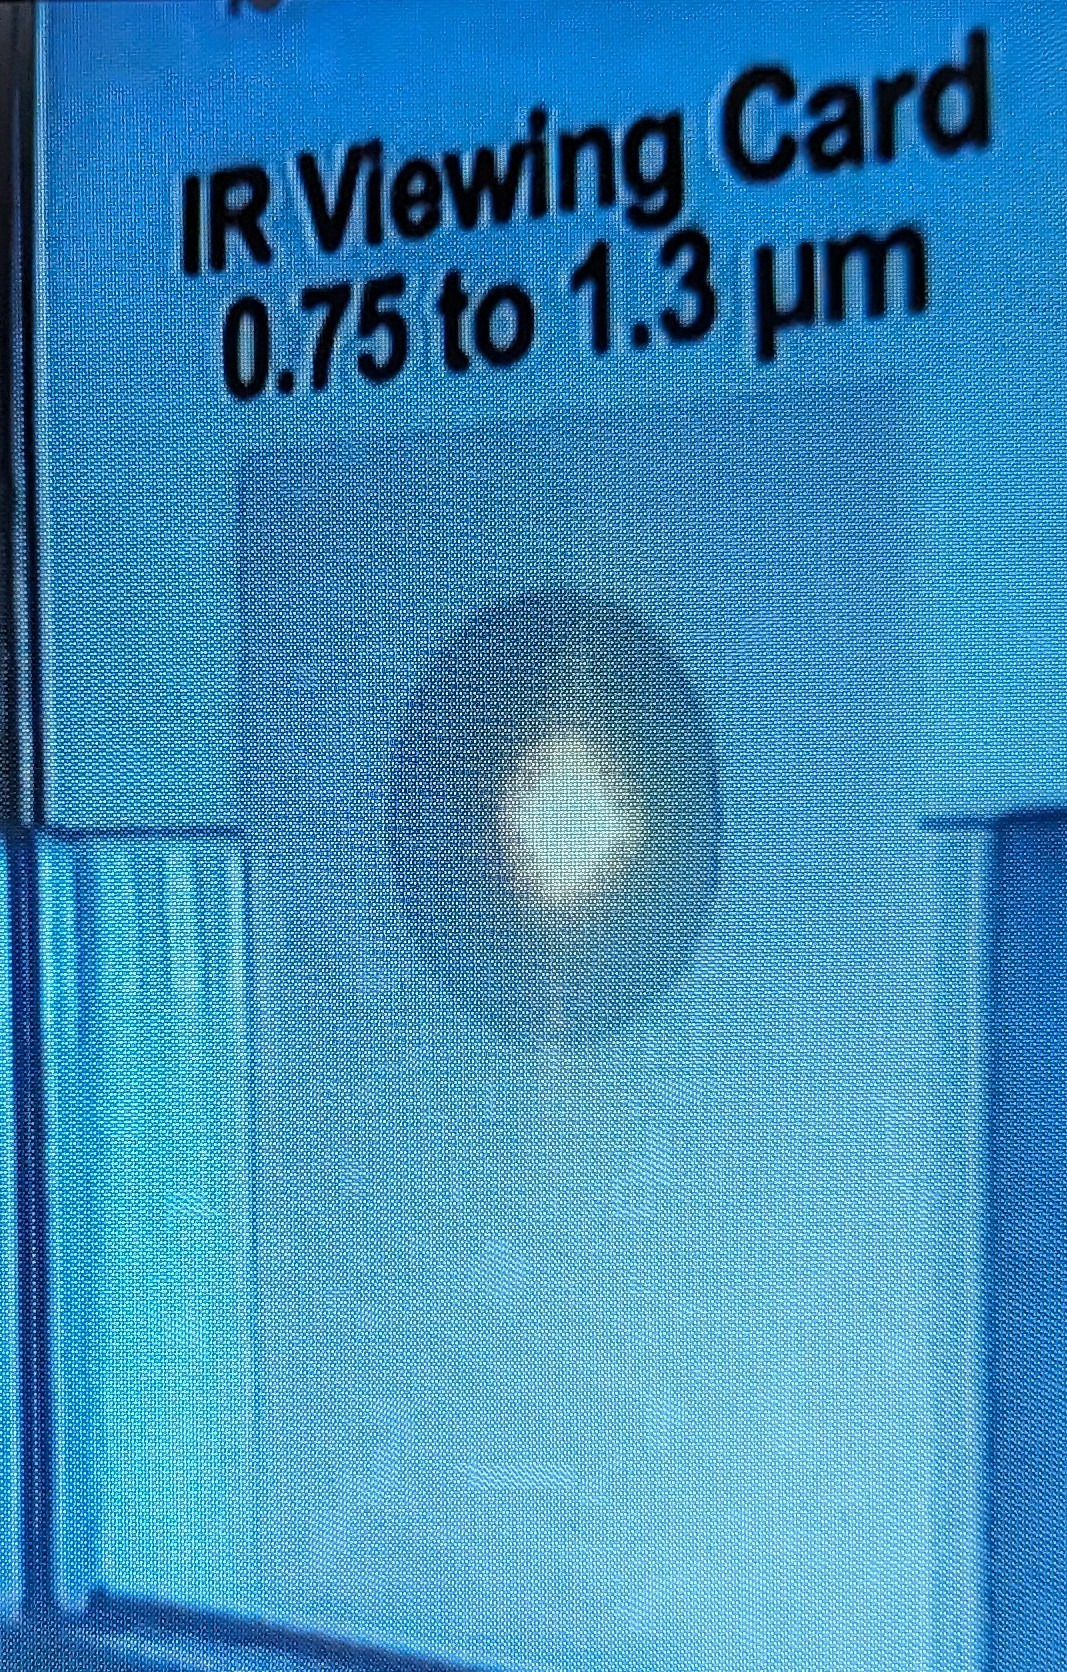
\includegraphics[width=0.6\textwidth]{bilder/under_threshold.jpg}
        \subcaption{$I = \qty{34.5}{\milli\ampere}$}
        \label{fig:under_threshold}
    \end{subfigure}
    \begin{subfigure}[c]{0.5\textwidth}
        \centering
        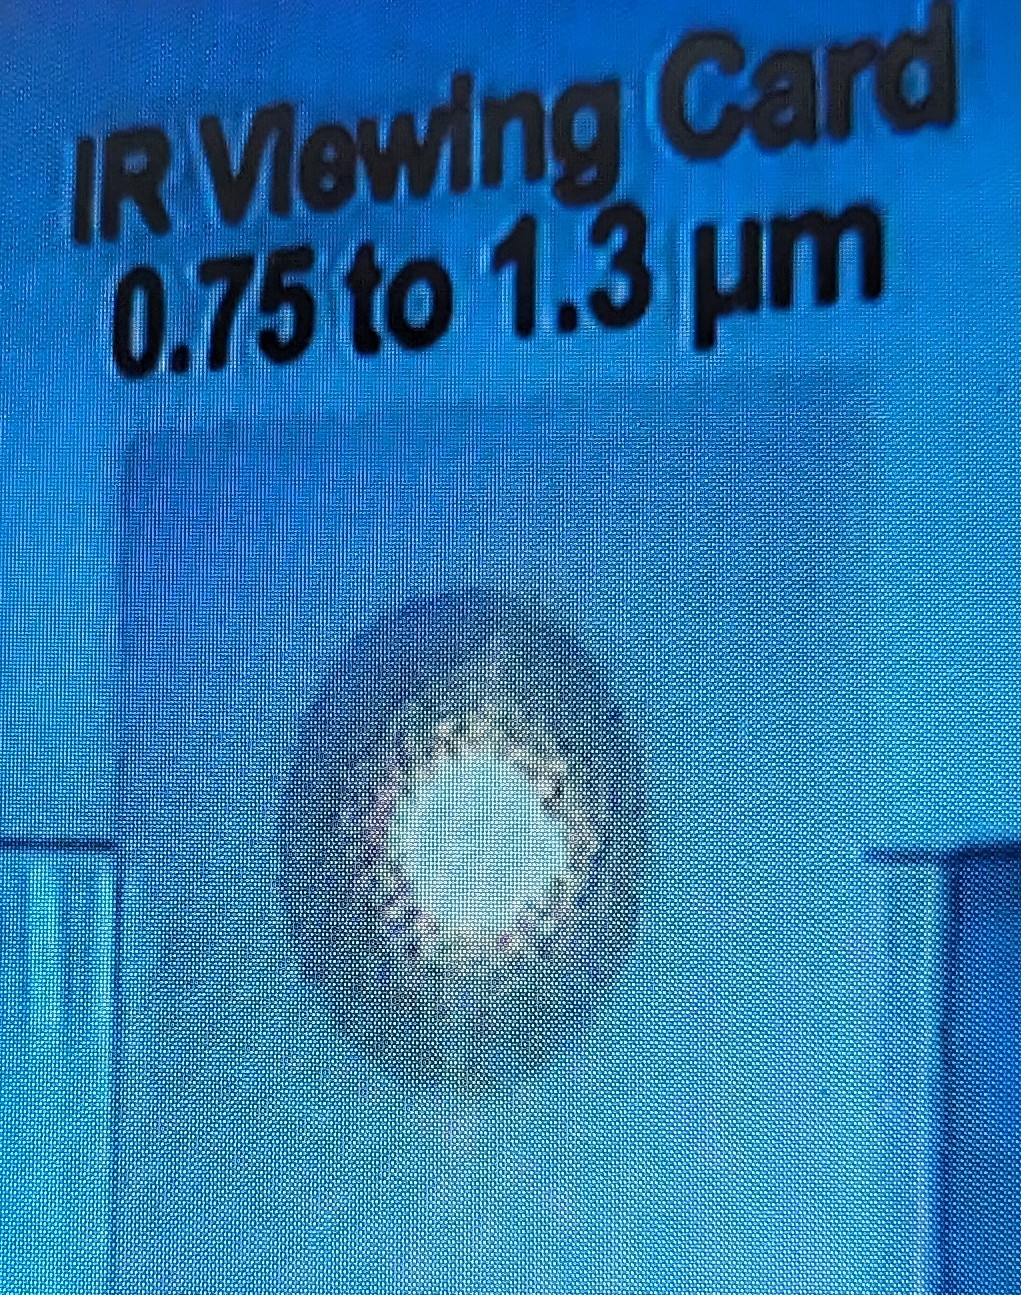
\includegraphics[width=0.6\textwidth]{bilder/above_threshold.jpg}
        \subcaption{$I = \qty{35.1}{\milli\ampere}$.}        
        \label{fig:above_threshold}
    \end{subfigure}
    \caption{Reflektion des Laserstrahls an einer Detektorkarte vor (\ref{fig:under_threshold}) und nach (\ref{fig:above_threshold}) Erreichen des Schwellenstromwerts. In \autoref{fig:above_threshold} ist um den Strahl herum ein getupftes Muster zu erkennen.}
\end{figure}

\section{Rubidiumfluoreszenz}

Wenn die Wellenlänge des Laserstrahls den Differenzen der Energieniveaus im Rubidium entsprechen, fängt das Rubidiumgas an zu fluoreszieren. Es wird angeregt und emittiert die Energie wieder
in Form von Photonen diffus im Raum. Eine Aufnahme dieses Effektes ist in \autoref{fig:fluoreszenz} zu sehen.\\

\begin{figure}
    \centering
    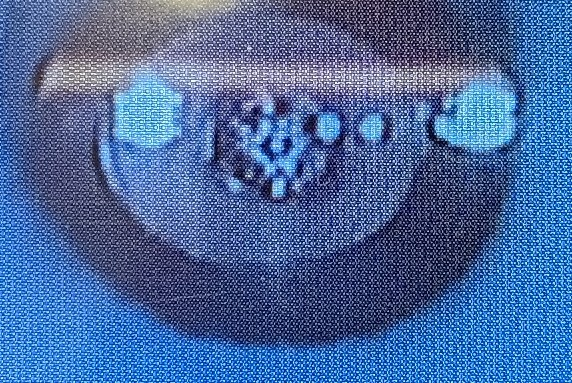
\includegraphics[width = 0.7\textwidth]{bilder/fluoreszenz.jpg}
    \caption{Fluoreszenz des Rubidium-Gasgemisch.}
    \label{fig:fluoreszenz}
\end{figure}

\section{Rubidium Absorptionsspektrum}

Für einen linear sinkenden (/ansteigenden) angelegten Strom werden mehrere Wellenlängen des Lasers durchlaufen. Es lässt sich nun ein zeitlicher Verlauf der gemessenen Intensität der Photodioden
messen. Es wird die Differenz der Photodioden verwendet, um Störeffekte zu vermindern und somit das reine Absorptionsspektrum des Rubidiumgases zu erhalten. Das aufgenommene Absorptionsspektrum ist in
\autoref{fig:rubidium} gezeigt. Zu sehen sind hier die in \autoref{fig:spektrum_rubidium} eingeführten Übergänge der Rubidium Isotope. Es lässt sich zusärtlich erkennen, dass die Peaks des Rb-85
Isotops in etwa $3$-Mal so groß sind, wie die des Rb-87 Isotops. Es liegt also etwa eine Verteilung von $\approx 33 \%$ Rb-87 und $\approx 66 \%$ Rb-85 vor.

\begin{figure}
    \centering
    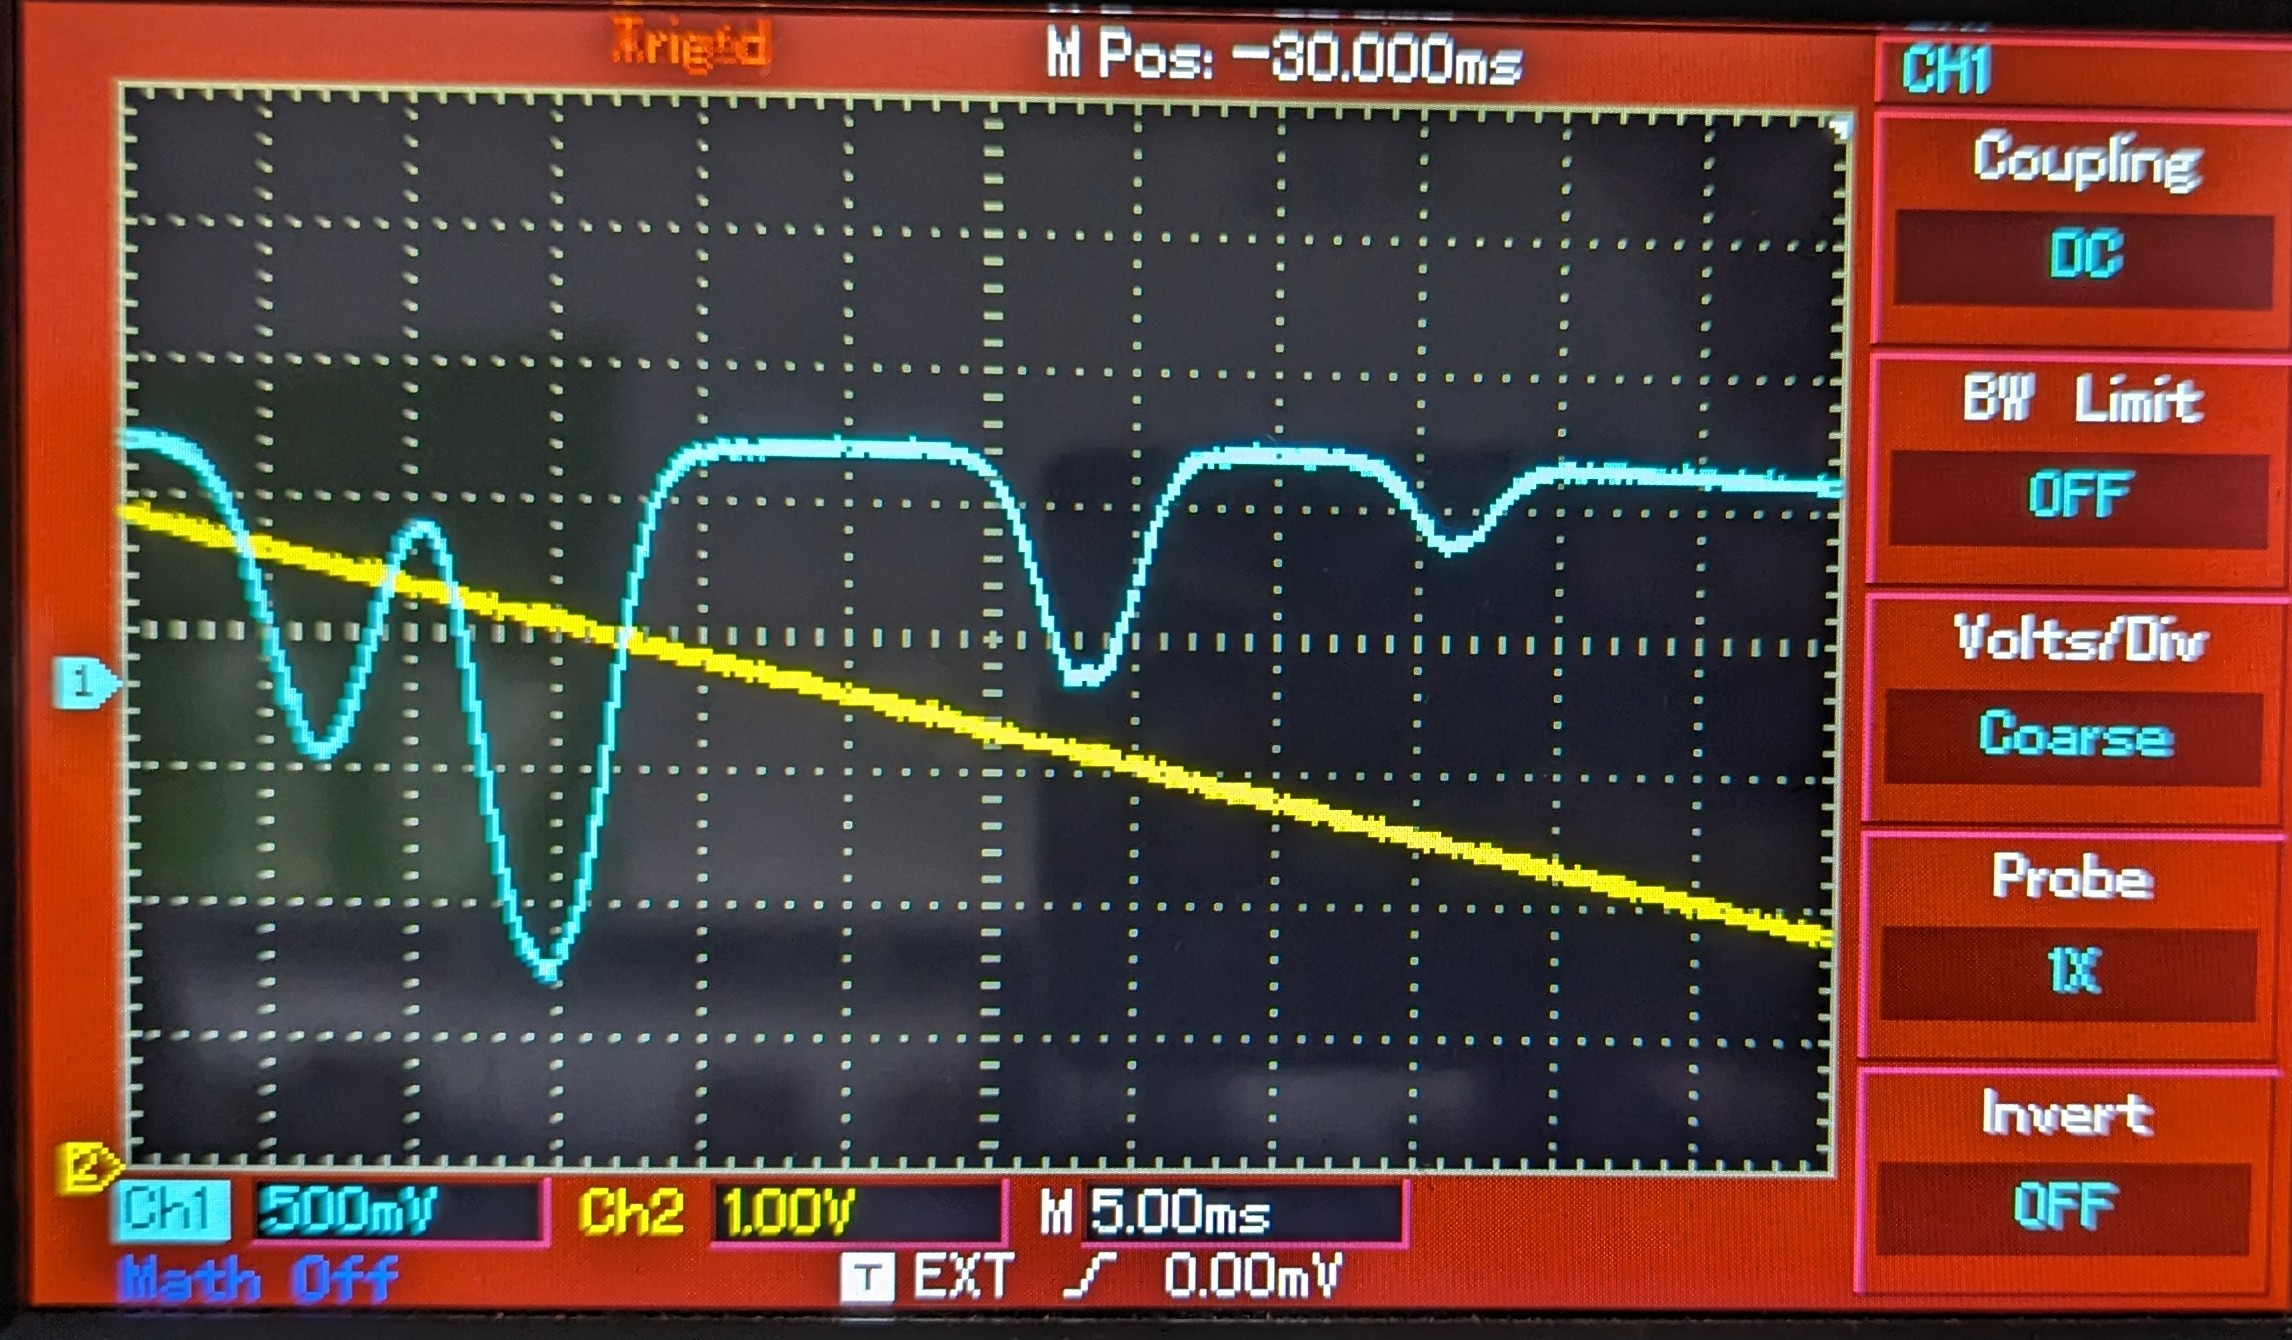
\includegraphics[width = 0.7\textwidth]{bilder/rubudium_abso.jpg}
    \caption{Absorptionsspektrum des Rubidiumgases.}
    \label{fig:rubidium}
\end{figure}